\documentclass[margin=2mm]{standalone}
\usepackage{tikz}
\usepackage{amsmath,amssymb,mathtools}
\begin{document}
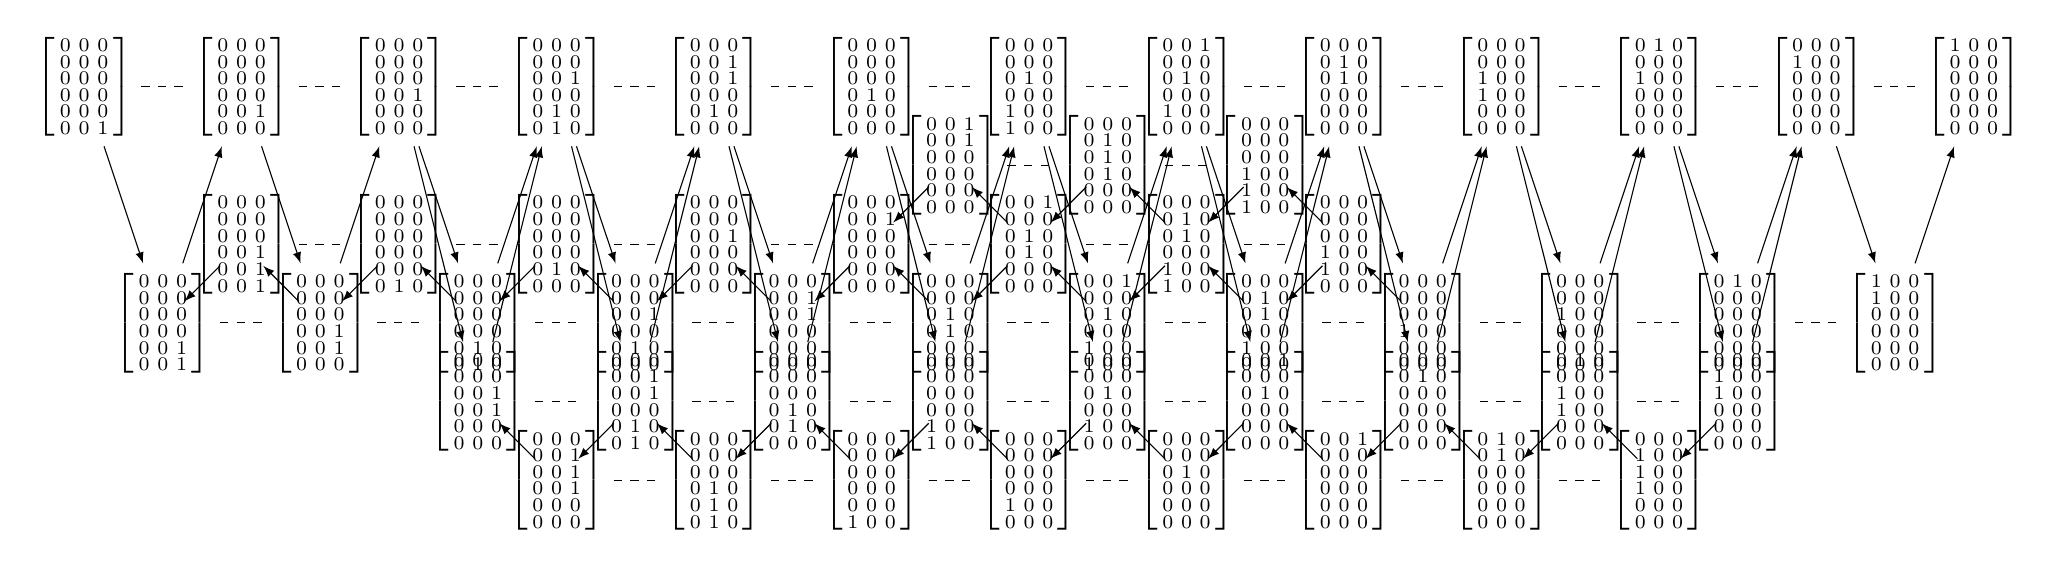
\begin{tikzpicture}
\node (t-0P5) at (0,3) [] {$\begin{bsmallmatrix}
 0 & 0 & 0\\
 0 & 0 & 0\\
 0 & 0 & 0\\
 0 & 0 & 0\\
 0 & 0 & 0\\
 0 & 0 & 1\\
\end{bsmallmatrix}$};
\node (t-1P5) at (2,3) [] {$\begin{bsmallmatrix}
 0 & 0 & 0\\
 0 & 0 & 0\\
 0 & 0 & 0\\
 0 & 0 & 0\\
 0 & 0 & 1\\
 0 & 0 & 0\\
\end{bsmallmatrix}$};
\node (t-2P5) at (4,3) [] {$\begin{bsmallmatrix}
 0 & 0 & 0\\
 0 & 0 & 0\\
 0 & 0 & 0\\
 0 & 0 & 1\\
 0 & 0 & 0\\
 0 & 0 & 0\\
\end{bsmallmatrix}$};
\node (t-3P5) at (6,3) [] {$\begin{bsmallmatrix}
 0 & 0 & 0\\
 0 & 0 & 0\\
 0 & 0 & 1\\
 0 & 0 & 0\\
 0 & 1 & 0\\
 0 & 1 & 0\\
\end{bsmallmatrix}$};
\node (t-4P5) at (8,3) [] {$\begin{bsmallmatrix}
 0 & 0 & 0\\
 0 & 0 & 1\\
 0 & 0 & 1\\
 0 & 0 & 0\\
 0 & 1 & 0\\
 0 & 0 & 0\\
\end{bsmallmatrix}$};
\node (t-5P5) at (10,3) [] {$\begin{bsmallmatrix}
 0 & 0 & 0\\
 0 & 0 & 0\\
 0 & 0 & 0\\
 0 & 1 & 0\\
 0 & 0 & 0\\
 0 & 0 & 0\\
\end{bsmallmatrix}$};
\node (t-6P5) at (12,3) [] {$\begin{bsmallmatrix}
 0 & 0 & 0\\
 0 & 0 & 0\\
 0 & 1 & 0\\
 0 & 0 & 0\\
 1 & 0 & 0\\
 1 & 0 & 0\\
\end{bsmallmatrix}$};
\node (t-7P5) at (14,3) [] {$\begin{bsmallmatrix}
 0 & 0 & 1\\
 0 & 0 & 0\\
 0 & 1 & 0\\
 0 & 0 & 0\\
 1 & 0 & 0\\
 0 & 0 & 0\\
\end{bsmallmatrix}$};
\node (t-8P5) at (16,3) [] {$\begin{bsmallmatrix}
 0 & 0 & 0\\
 0 & 1 & 0\\
 0 & 1 & 0\\
 0 & 0 & 0\\
 0 & 0 & 0\\
 0 & 0 & 0\\
\end{bsmallmatrix}$};
\node (t-9P5) at (18,3) [] {$\begin{bsmallmatrix}
 0 & 0 & 0\\
 0 & 0 & 0\\
 1 & 0 & 0\\
 1 & 0 & 0\\
 0 & 0 & 0\\
 0 & 0 & 0\\
\end{bsmallmatrix}$};
\node (t-10P5) at (20,3) [] {$\begin{bsmallmatrix}
 0 & 1 & 0\\
 0 & 0 & 0\\
 1 & 0 & 0\\
 0 & 0 & 0\\
 0 & 0 & 0\\
 0 & 0 & 0\\
\end{bsmallmatrix}$};
\node (t-11P5) at (22,3) [] {$\begin{bsmallmatrix}
 0 & 0 & 0\\
 1 & 0 & 0\\
 0 & 0 & 0\\
 0 & 0 & 0\\
 0 & 0 & 0\\
 0 & 0 & 0\\
\end{bsmallmatrix}$};
\node (t-12P5) at (24,3) [] {$\begin{bsmallmatrix}
 1 & 0 & 0\\
 0 & 0 & 0\\
 0 & 0 & 0\\
 0 & 0 & 0\\
 0 & 0 & 0\\
 0 & 0 & 0\\
\end{bsmallmatrix}$};
\node (t-0P4) at (1,0) [] {$\begin{bsmallmatrix}
 0 & 0 & 0\\
 0 & 0 & 0\\
 0 & 0 & 0\\
 0 & 0 & 0\\
 0 & 0 & 1\\
 0 & 0 & 1\\
\end{bsmallmatrix}$};
\node (t-1P4) at (3,0) [] {$\begin{bsmallmatrix}
 0 & 0 & 0\\
 0 & 0 & 0\\
 0 & 0 & 0\\
 0 & 0 & 1\\
 0 & 0 & 1\\
 0 & 0 & 0\\
\end{bsmallmatrix}$};
\node (t-2P4) at (5,0) [] {$\begin{bsmallmatrix}
 0 & 0 & 0\\
 0 & 0 & 0\\
 0 & 0 & 0\\
 0 & 0 & 0\\
 0 & 1 & 0\\
 0 & 1 & 0\\
\end{bsmallmatrix}$};
\node (t-3P4) at (7,0) [] {$\begin{bsmallmatrix}
 0 & 0 & 0\\
 0 & 0 & 0\\
 0 & 0 & 1\\
 0 & 0 & 0\\
 0 & 1 & 0\\
 0 & 0 & 0\\
\end{bsmallmatrix}$};
\node (t-4P4) at (9,0) [] {$\begin{bsmallmatrix}
 0 & 0 & 0\\
 0 & 0 & 1\\
 0 & 0 & 1\\
 0 & 0 & 0\\
 0 & 0 & 0\\
 0 & 0 & 0\\
\end{bsmallmatrix}$};
\node (t-5P4) at (11,0) [] {$\begin{bsmallmatrix}
 0 & 0 & 0\\
 0 & 0 & 0\\
 0 & 1 & 0\\
 0 & 1 & 0\\
 0 & 0 & 0\\
 0 & 0 & 0\\
\end{bsmallmatrix}$};
\node (t-6P4) at (13,0) [] {$\begin{bsmallmatrix}
 0 & 0 & 1\\
 0 & 0 & 0\\
 0 & 1 & 0\\
 0 & 0 & 0\\
 1 & 0 & 0\\
 1 & 0 & 0\\
\end{bsmallmatrix}$};
\node (t-7P4) at (15,0) [] {$\begin{bsmallmatrix}
 0 & 0 & 0\\
 0 & 1 & 0\\
 0 & 1 & 0\\
 0 & 0 & 0\\
 1 & 0 & 0\\
 0 & 0 & 0\\
\end{bsmallmatrix}$};
\node (t-8P4) at (17,0) [] {$\begin{bsmallmatrix}
 0 & 0 & 0\\
 0 & 0 & 0\\
 0 & 0 & 0\\
 1 & 0 & 0\\
 0 & 0 & 0\\
 0 & 0 & 0\\
\end{bsmallmatrix}$};
\node (t-9P4) at (19,0) [] {$\begin{bsmallmatrix}
 0 & 0 & 0\\
 0 & 0 & 0\\
 1 & 0 & 0\\
 0 & 0 & 0\\
 0 & 0 & 0\\
 0 & 0 & 0\\
\end{bsmallmatrix}$};
\node (t-10P4) at (21,0) [] {$\begin{bsmallmatrix}
 0 & 1 & 0\\
 0 & 0 & 0\\
 0 & 0 & 0\\
 0 & 0 & 0\\
 0 & 0 & 0\\
 0 & 0 & 0\\
\end{bsmallmatrix}$};
\node (t-11P4) at (23,0) [] {$\begin{bsmallmatrix}
 1 & 0 & 0\\
 1 & 0 & 0\\
 0 & 0 & 0\\
 0 & 0 & 0\\
 0 & 0 & 0\\
 0 & 0 & 0\\
\end{bsmallmatrix}$};
\node (t-0P3) at (2,1) [] {$\begin{bsmallmatrix}
 0 & 0 & 0\\
 0 & 0 & 0\\
 0 & 0 & 0\\
 0 & 0 & 1\\
 0 & 0 & 1\\
 0 & 0 & 1\\
\end{bsmallmatrix}$};
\node (t-1P3) at (4,1) [] {$\begin{bsmallmatrix}
 0 & 0 & 0\\
 0 & 0 & 0\\
 0 & 0 & 0\\
 0 & 0 & 0\\
 0 & 0 & 0\\
 0 & 1 & 0\\
\end{bsmallmatrix}$};
\node (t-2P3) at (6,1) [] {$\begin{bsmallmatrix}
 0 & 0 & 0\\
 0 & 0 & 0\\
 0 & 0 & 0\\
 0 & 0 & 0\\
 0 & 1 & 0\\
 0 & 0 & 0\\
\end{bsmallmatrix}$};
\node (t-3P3) at (8,1) [] {$\begin{bsmallmatrix}
 0 & 0 & 0\\
 0 & 0 & 0\\
 0 & 0 & 1\\
 0 & 0 & 0\\
 0 & 0 & 0\\
 0 & 0 & 0\\
\end{bsmallmatrix}$};
\node (t-4P3) at (10,1) [] {$\begin{bsmallmatrix}
 0 & 0 & 0\\
 0 & 0 & 1\\
 0 & 0 & 0\\
 0 & 0 & 0\\
 0 & 0 & 0\\
 0 & 0 & 0\\
\end{bsmallmatrix}$};
\node (t-5P3) at (12,1) [] {$\begin{bsmallmatrix}
 0 & 0 & 1\\
 0 & 0 & 0\\
 0 & 1 & 0\\
 0 & 1 & 0\\
 0 & 0 & 0\\
 0 & 0 & 0\\
\end{bsmallmatrix}$};
\node (t-6P3) at (14,1) [] {$\begin{bsmallmatrix}
 0 & 0 & 0\\
 0 & 1 & 0\\
 0 & 1 & 0\\
 0 & 0 & 0\\
 1 & 0 & 0\\
 1 & 0 & 0\\
\end{bsmallmatrix}$};
\node (t-7P3) at (16,1) [] {$\begin{bsmallmatrix}
 0 & 0 & 0\\
 0 & 0 & 0\\
 0 & 0 & 0\\
 1 & 0 & 0\\
 1 & 0 & 0\\
 0 & 0 & 0\\
\end{bsmallmatrix}$};
\node (t-0P2) at (5,-1) [] {$\begin{bsmallmatrix}
 0 & 0 & 0\\
 0 & 0 & 0\\
 0 & 0 & 1\\
 0 & 0 & 1\\
 0 & 0 & 0\\
 0 & 0 & 0\\
\end{bsmallmatrix}$};
\node (t-1P2) at (7,-1) [] {$\begin{bsmallmatrix}
 0 & 0 & 0\\
 0 & 0 & 1\\
 0 & 0 & 1\\
 0 & 0 & 0\\
 0 & 1 & 0\\
 0 & 1 & 0\\
\end{bsmallmatrix}$};
\node (t-2P2) at (9,-1) [] {$\begin{bsmallmatrix}
 0 & 0 & 0\\
 0 & 0 & 0\\
 0 & 0 & 0\\
 0 & 1 & 0\\
 0 & 1 & 0\\
 0 & 0 & 0\\
\end{bsmallmatrix}$};
\node (t-3P2) at (11,-1) [] {$\begin{bsmallmatrix}
 0 & 0 & 0\\
 0 & 0 & 0\\
 0 & 0 & 0\\
 0 & 0 & 0\\
 1 & 0 & 0\\
 1 & 0 & 0\\
\end{bsmallmatrix}$};
\node (t-4P2) at (13,-1) [] {$\begin{bsmallmatrix}
 0 & 0 & 0\\
 0 & 0 & 0\\
 0 & 1 & 0\\
 0 & 0 & 0\\
 1 & 0 & 0\\
 0 & 0 & 0\\
\end{bsmallmatrix}$};
\node (t-5P2) at (15,-1) [] {$\begin{bsmallmatrix}
 0 & 0 & 1\\
 0 & 0 & 0\\
 0 & 1 & 0\\
 0 & 0 & 0\\
 0 & 0 & 0\\
 0 & 0 & 0\\
\end{bsmallmatrix}$};
\node (t-6P2) at (17,-1) [] {$\begin{bsmallmatrix}
 0 & 0 & 0\\
 0 & 1 & 0\\
 0 & 0 & 0\\
 0 & 0 & 0\\
 0 & 0 & 0\\
 0 & 0 & 0\\
\end{bsmallmatrix}$};
\node (t-7P2) at (19,-1) [] {$\begin{bsmallmatrix}
 0 & 1 & 0\\
 0 & 0 & 0\\
 1 & 0 & 0\\
 1 & 0 & 0\\
 0 & 0 & 0\\
 0 & 0 & 0\\
\end{bsmallmatrix}$};
\node (t-8P2) at (21,-1) [] {$\begin{bsmallmatrix}
 0 & 0 & 0\\
 1 & 0 & 0\\
 1 & 0 & 0\\
 0 & 0 & 0\\
 0 & 0 & 0\\
 0 & 0 & 0\\
\end{bsmallmatrix}$};
\node (t-0P1) at (6,-2) [] {$\begin{bsmallmatrix}
 0 & 0 & 0\\
 0 & 0 & 1\\
 0 & 0 & 1\\
 0 & 0 & 1\\
 0 & 0 & 0\\
 0 & 0 & 0\\
\end{bsmallmatrix}$};
\node (t-1P1) at (8,-2) [] {$\begin{bsmallmatrix}
 0 & 0 & 0\\
 0 & 0 & 0\\
 0 & 0 & 0\\
 0 & 1 & 0\\
 0 & 1 & 0\\
 0 & 1 & 0\\
\end{bsmallmatrix}$};
\node (t-2P1) at (10,-2) [] {$\begin{bsmallmatrix}
 0 & 0 & 0\\
 0 & 0 & 0\\
 0 & 0 & 0\\
 0 & 0 & 0\\
 0 & 0 & 0\\
 1 & 0 & 0\\
\end{bsmallmatrix}$};
\node (t-3P1) at (12,-2) [] {$\begin{bsmallmatrix}
 0 & 0 & 0\\
 0 & 0 & 0\\
 0 & 0 & 0\\
 0 & 0 & 0\\
 1 & 0 & 0\\
 0 & 0 & 0\\
\end{bsmallmatrix}$};
\node (t-4P1) at (14,-2) [] {$\begin{bsmallmatrix}
 0 & 0 & 0\\
 0 & 0 & 0\\
 0 & 1 & 0\\
 0 & 0 & 0\\
 0 & 0 & 0\\
 0 & 0 & 0\\
\end{bsmallmatrix}$};
\node (t-5P1) at (16,-2) [] {$\begin{bsmallmatrix}
 0 & 0 & 1\\
 0 & 0 & 0\\
 0 & 0 & 0\\
 0 & 0 & 0\\
 0 & 0 & 0\\
 0 & 0 & 0\\
\end{bsmallmatrix}$};
\node (t-6P1) at (18,-2) [] {$\begin{bsmallmatrix}
 0 & 1 & 0\\
 0 & 1 & 0\\
 0 & 0 & 0\\
 0 & 0 & 0\\
 0 & 0 & 0\\
 0 & 0 & 0\\
\end{bsmallmatrix}$};
\node (t-7P1) at (20,-2) [] {$\begin{bsmallmatrix}
 0 & 0 & 0\\
 1 & 0 & 0\\
 1 & 0 & 0\\
 1 & 0 & 0\\
 0 & 0 & 0\\
 0 & 0 & 0\\
\end{bsmallmatrix}$};
\node (t-0P0) at (11,2) [] {$\begin{bsmallmatrix}
 0 & 0 & 1\\
 0 & 0 & 1\\
 0 & 0 & 0\\
 0 & 0 & 0\\
 0 & 0 & 0\\
 0 & 0 & 0\\
\end{bsmallmatrix}$};
\node (t-1P0) at (13,2) [] {$\begin{bsmallmatrix}
 0 & 0 & 0\\
 0 & 1 & 0\\
 0 & 1 & 0\\
 0 & 1 & 0\\
 0 & 0 & 0\\
 0 & 0 & 0\\
\end{bsmallmatrix}$};
\node (t-2P0) at (15,2) [] {$\begin{bsmallmatrix}
 0 & 0 & 0\\
 0 & 0 & 0\\
 0 & 0 & 0\\
 1 & 0 & 0\\
 1 & 0 & 0\\
 1 & 0 & 0\\
\end{bsmallmatrix}$};
\draw[-latex] (t-0P5) -- (t-0P4);
\draw[-latex] (t-1P5) -- (t-1P4);
\draw[-latex] (t-2P5) -- (t-0P2);
\draw[-latex] (t-2P5) -- (t-2P4);
\draw[-latex] (t-3P5) -- (t-3P4);
\draw[-latex] (t-3P5) -- (t-1P2);
\draw[-latex] (t-4P5) -- (t-4P4);
\draw[-latex] (t-4P5) -- (t-2P2);
\draw[-latex] (t-5P5) -- (t-5P4);
\draw[-latex] (t-5P5) -- (t-3P2);
\draw[-latex] (t-6P5) -- (t-6P4);
\draw[-latex] (t-6P5) -- (t-4P2);
\draw[-latex] (t-7P5) -- (t-7P4);
\draw[-latex] (t-7P5) -- (t-5P2);
\draw[-latex] (t-8P5) -- (t-8P4);
\draw[-latex] (t-8P5) -- (t-6P2);
\draw[-latex] (t-9P5) -- (t-9P4);
\draw[-latex] (t-9P5) -- (t-7P2);
\draw[-latex] (t-10P5) -- (t-10P4);
\draw[-latex] (t-10P5) -- (t-8P2);
\draw[-latex] (t-11P5) -- (t-11P4);
\draw[-latex] (t-0P4) -- (t-0P3);
\draw[-latex] (t-0P4) -- (t-1P5);
\draw[-latex] (t-1P4) -- (t-1P3);
\draw[-latex] (t-1P4) -- (t-2P5);
\draw[-latex] (t-2P4) -- (t-2P3);
\draw[-latex] (t-2P4) -- (t-3P5);
\draw[-latex] (t-3P4) -- (t-3P3);
\draw[-latex] (t-3P4) -- (t-4P5);
\draw[-latex] (t-4P4) -- (t-4P3);
\draw[-latex] (t-4P4) -- (t-5P5);
\draw[-latex] (t-5P4) -- (t-5P3);
\draw[-latex] (t-5P4) -- (t-6P5);
\draw[-latex] (t-6P4) -- (t-6P3);
\draw[-latex] (t-6P4) -- (t-7P5);
\draw[-latex] (t-7P4) -- (t-7P3);
\draw[-latex] (t-7P4) -- (t-8P5);
\draw[-latex] (t-8P4) -- (t-9P5);
\draw[-latex] (t-9P4) -- (t-10P5);
\draw[-latex] (t-10P4) -- (t-11P5);
\draw[-latex] (t-11P4) -- (t-12P5);
\draw[-latex] (t-0P3) -- (t-1P4);
\draw[-latex] (t-1P3) -- (t-2P4);
\draw[-latex] (t-2P3) -- (t-3P4);
\draw[-latex] (t-3P3) -- (t-4P4);
\draw[-latex] (t-4P3) -- (t-0P0);
\draw[-latex] (t-4P3) -- (t-5P4);
\draw[-latex] (t-5P3) -- (t-1P0);
\draw[-latex] (t-5P3) -- (t-6P4);
\draw[-latex] (t-6P3) -- (t-2P0);
\draw[-latex] (t-6P3) -- (t-7P4);
\draw[-latex] (t-7P3) -- (t-8P4);
\draw[-latex] (t-0P2) -- (t-0P1);
\draw[-latex] (t-0P2) -- (t-3P5);
\draw[-latex] (t-1P2) -- (t-4P5);
\draw[-latex] (t-1P2) -- (t-1P1);
\draw[-latex] (t-2P2) -- (t-5P5);
\draw[-latex] (t-2P2) -- (t-2P1);
\draw[-latex] (t-3P2) -- (t-6P5);
\draw[-latex] (t-3P2) -- (t-3P1);
\draw[-latex] (t-4P2) -- (t-7P5);
\draw[-latex] (t-4P2) -- (t-4P1);
\draw[-latex] (t-5P2) -- (t-8P5);
\draw[-latex] (t-5P2) -- (t-5P1);
\draw[-latex] (t-6P2) -- (t-9P5);
\draw[-latex] (t-6P2) -- (t-6P1);
\draw[-latex] (t-7P2) -- (t-10P5);
\draw[-latex] (t-7P2) -- (t-7P1);
\draw[-latex] (t-8P2) -- (t-11P5);
\draw[-latex] (t-0P1) -- (t-1P2);
\draw[-latex] (t-1P1) -- (t-2P2);
\draw[-latex] (t-2P1) -- (t-3P2);
\draw[-latex] (t-3P1) -- (t-4P2);
\draw[-latex] (t-4P1) -- (t-5P2);
\draw[-latex] (t-5P1) -- (t-6P2);
\draw[-latex] (t-6P1) -- (t-7P2);
\draw[-latex] (t-7P1) -- (t-8P2);
\draw[-latex] (t-0P0) -- (t-5P3);
\draw[-latex] (t-1P0) -- (t-6P3);
\draw[-latex] (t-2P0) -- (t-7P3);
\draw[dashed] (t-0P5)--(t-1P5);
\draw[dashed] (t-1P5)--(t-2P5);
\draw[dashed] (t-2P5)--(t-3P5);
\draw[dashed] (t-3P5)--(t-4P5);
\draw[dashed] (t-4P5)--(t-5P5);
\draw[dashed] (t-5P5)--(t-6P5);
\draw[dashed] (t-6P5)--(t-7P5);
\draw[dashed] (t-7P5)--(t-8P5);
\draw[dashed] (t-8P5)--(t-9P5);
\draw[dashed] (t-9P5)--(t-10P5);
\draw[dashed] (t-10P5)--(t-11P5);
\draw[dashed] (t-11P5)--(t-12P5);
\draw[dashed] (t-0P4)--(t-1P4);
\draw[dashed] (t-1P4)--(t-2P4);
\draw[dashed] (t-2P4)--(t-3P4);
\draw[dashed] (t-3P4)--(t-4P4);
\draw[dashed] (t-4P4)--(t-5P4);
\draw[dashed] (t-5P4)--(t-6P4);
\draw[dashed] (t-6P4)--(t-7P4);
\draw[dashed] (t-7P4)--(t-8P4);
\draw[dashed] (t-8P4)--(t-9P4);
\draw[dashed] (t-9P4)--(t-10P4);
\draw[dashed] (t-10P4)--(t-11P4);
\draw[dashed] (t-0P3)--(t-1P3);
\draw[dashed] (t-1P3)--(t-2P3);
\draw[dashed] (t-2P3)--(t-3P3);
\draw[dashed] (t-3P3)--(t-4P3);
\draw[dashed] (t-4P3)--(t-5P3);
\draw[dashed] (t-5P3)--(t-6P3);
\draw[dashed] (t-6P3)--(t-7P3);
\draw[dashed] (t-0P2)--(t-1P2);
\draw[dashed] (t-1P2)--(t-2P2);
\draw[dashed] (t-2P2)--(t-3P2);
\draw[dashed] (t-3P2)--(t-4P2);
\draw[dashed] (t-4P2)--(t-5P2);
\draw[dashed] (t-5P2)--(t-6P2);
\draw[dashed] (t-6P2)--(t-7P2);
\draw[dashed] (t-7P2)--(t-8P2);
\draw[dashed] (t-0P1)--(t-1P1);
\draw[dashed] (t-1P1)--(t-2P1);
\draw[dashed] (t-2P1)--(t-3P1);
\draw[dashed] (t-3P1)--(t-4P1);
\draw[dashed] (t-4P1)--(t-5P1);
\draw[dashed] (t-5P1)--(t-6P1);
\draw[dashed] (t-6P1)--(t-7P1);
\draw[dashed] (t-0P0)--(t-1P0);
\draw[dashed] (t-1P0)--(t-2P0);
\end{tikzpicture}\end{document}